%%%%%%%%%%%%%%%%%%%% author.tex %%%%%%%%%%%%%%%%%%%%%%%%%%%%%%%%%%%
%
% sample root file for your "contribution" to a contributed volume
%
% Use this file as a template for your own input.
%
%%%%%%%%%%%%%%%% Springer %%%%%%%%%%%%%%%%%%%%%%%%%%%%%%%%%%
% RECOMMENDED %%%%%%%%%%%%%%%%%%%%%%%%%%%%%%%%%%%%%%%%%%%%%%%%%%%
\documentclass[graybox]{svmult}
% choose options for [] as required from the list
% in the Reference Guide
\usepackage{type1cm}        % activate if the above 3 fonts are
                            % not available on your system
%
\usepackage{makeidx}         % allows index generation
%\usepackage{graphicx}        % standard LaTeX graphics tool
                             % when including Fig.~files
\usepackage{multicol}        % used for the two-column index
\usepackage[bottom]{footmisc}% places footnotes at page bottom
\usepackage{newtxtext}       % 
\usepackage{newtxmath}       % selects Times Roman as basic font
% see the list of further useful packages
% in the Reference Guide
%\makeindex             % used for the subject index
                       % please use the style svind.ist with
                       % your makeindex program
%%%%%%%%%%%%%%%%%%%%%%%%%%%%%%%%%%%%%%%%%%%%%%%%%%%%%%%%%%%%%%%%%%%%%%%%%%%%%%%%%%%%%%%%%
% \usepackage{amsmath}
% \usepackage{ascmac}
\usepackage[dvipdfmx]{graphicx}  % for EPS and PDF 
% \usepackage{url}
\usepackage{fancyvrb}
\usepackage{multirow}
% \usepackage{makeidx}
% \usepackage{float}
% \usepackage[dvipdfmx]{color}
% \usepackage{ulem}
% \usepackage[switch*,pagewise]{lineno}
% \usepackage[dvipdfm,bookmarkstype=toc,urlcolor=black,%
%     linkcolor=black,citecolor=black,bookmarks=false]{hyperref}
% \usepackage{fancyhdr}

\usepackage{listings}
\lstset{%
 language={C},
% basicstyle={\scriptsize},%
% identifierstyle={\scriptsize},%
 basicstyle={\small},%
 identifierstyle={\small},%
% commentstyle={\small\itshape},%
%commentstyle={\scriptsize},%
commentstyle={\small},%
 keywordstyle={\small\bfseries},%
 ndkeywordstyle={\small},%
stringstyle={\small\ttfamily},
 frame={tb},
 breaklines=true,
 columns=[l]{fullflexible},%
 numbers=left,%
 xrightmargin=1zw,%
 xleftmargin=1.5zw,%
 numberstyle={\small},%
 stepnumber=1,
 numbersep=1zw,%
% lineskip=-0.1ex%
}

\def\XMP{XcalableMP}
\def\OMP{OpenMP}
\def\HPF{HPF}
\def\CAF{Co-array Fortran}
\def\MPI{MPI}
\def\Fort{Fortran}
\def\C{C}
\def\XMPF{XcalableMP Fortran}
\def\XMPC{XcalableMP C}

\def\openb{{\it [}}
\def\closeb{{\it ]}}
\def\bsquare{\rule[-2pt]{5pt}{10pt}}

\def\|{\verb|}

%\newenvironment{myfigure}{\begin{figure}[ht]\begin{center}}{\end{center}\end{figure}}

\def\Directive#1{{\tt #1}\index{#1@{\tt #1}}\index{Directive!#1@{\tt #1}}}

%\def\Syntax#1{\index{{\tt #1}}\index{Syntax!{\tt #1}}}
\def\Syntax#1{\index{Syntax!#1@{\tt #1}}}

\def\Term#1{{#1}\index{#1}}

%\def\Example#1{\index{#1}\index{Example!{\tt #1}}}
\def\Example#1{\index{Example!#1@{\tt #1}}}

\def\Intrinsic#1{\index{#1@{\tt #1}}\index{Intrinsic and Library Procedures!#1@{\tt #1}}}

\DefineVerbatimEnvironment{Fexample}{Verbatim}{numbers=left,numbersep=3pt,stepnumber=5,%
frame=single,label=\Fort}
\DefineVerbatimEnvironment{FexampleR}{Verbatim}{numbers=right,numbersep=3pt,stepnumber=5,%
frame=single,label=\Fort}

\DefineVerbatimEnvironment{Cexample}{Verbatim}{numbers=left,numbersep=3pt,stepnumber=5,%
frame=single,label=\C}
\DefineVerbatimEnvironment{CexampleR}{Verbatim}{numbers=right,numbersep=3pt,stepnumber=5,%
frame=single,label=\C}

\DefineVerbatimEnvironment{XFexample}{Verbatim}{numbers=left,numbersep=3pt,stepnumber=5,%
frame=single,label=\XMPF}
\DefineVerbatimEnvironment{XFexampleR}{Verbatim}{numbers=right,numbersep=3pt,stepnumber=5,%
frame=single,label=\XMPF}

\DefineVerbatimEnvironment{XCexample}{Verbatim}{numbers=left,numbersep=3pt,stepnumber=5,%
frame=single,label=\XMPC}
\DefineVerbatimEnvironment{XCexampleR}{Verbatim}{numbers=right,numbersep=3pt,stepnumber=5,%
frame=single,label=\XMPC}

\DefineVerbatimEnvironment{MPICexample}{Verbatim}{numbers=right,numbersep=3pt,stepnumber=5,%
frame=single,label=MPI C}
\DefineVerbatimEnvironment{MPIFexample}{Verbatim}{numbers=right,numbersep=3pt,stepnumber=5,%
frame=single,label=MPI Fortran}


\setcounter{secnumdepth}{4}
\setcounter{tocdepth}{3}
\setcounter{totalnumber}{6}
\usepackage{fancyhdr}

\let\olditemize\itemize
\renewcommand{\itemize}{
   \olditemize
   \setlength{\itemsep}{8pt}
   \setlength{\parskip}{0pt}
   \setlength{\parsep}{0pt}
}

% \parindent = 0pt
% \hoffset=0cm
% \oddsidemargin=0cm
% \evensidemargin=0cm
% \textwidth=16cm
% \topmargin=-1cm
% \voffset=0cm
% \textheight=24cm

\def\progenv{\baselineskip=10pt\tt\progspecial{`}\parindent=0.3cm}
\def\shellenv{\baselineskip=10pt\tt\progspecial{`}\parindent=0.3cm\nolineno}

\renewcommand{\topfraction}{.99}
\renewcommand{\bottomfraction}{.99}

\def\openb{{\it [}}
\def\closeb{{\it ]}}
\def\XMP{XMP}
\def\XACC{XACC}
\def\OACC{OpenACC}
\def\OMP{OpenMP}
\def\XMPF{XcalableMP Fortran}
\def\XMPC{XcalableMP C}
\def\XACCF{XcalableACC Fortran}
\def\XACCC{XcalableACC C}
\def\Syntax#1{\index{Syntax!#1@{\tt #1}}}
\def\Example#1{\index{Example!#1@{\tt #1}}}
%
\def\phrule{\vspace{0.2cm}\hrule\vspace{0.05cm}\hrule}
\def\qhrule{\vspace{0.2cm}\hrule}
\def\dhrule{\hrule\vspace{0.05cm}\hrule}
\def\bsquare{\rule[-2pt]{5pt}{10pt}}
%
\newenvironment{mytable}[3]{\begin{table}[ht]\caption{#1}\label{#2}\vspace*{-0.3cm}\begin{center}\begin{tabular}{#3}}{\end{tabular}\end{center}\end{table}}
\newenvironment{myfigure}{\begin{figure}[ht]\begin{center}}{\end{center}\end{figure}}
%
\DefineVerbatimEnvironment{XACCFexampleL}{Verbatim}{numbers=left,numbersep=3pt,stepnumber=5,frame=single,label=\XACCF}
\DefineVerbatimEnvironment{XACCCexampleR}{Verbatim}{numbers=right,numbersep=3pt,stepnumber=5,frame=single,label=\XACCC}
\DefineVerbatimEnvironment{XACCCexampleL}{Verbatim}{numbers=left,numbersep=3pt,stepnumber=5,frame=single,label=\XACCC}


%%%%%%%%%%%%%%%%%%%%%%%%%%%%%%%%%%%%%%%%%%%%%%%%%%%%%%%%%%%%%%%%%%%%%%%%%%%%%%%%%%%%%%%%%
\begin{document}



\title*{XcalableACC: an Integration of XcalableMP and OpenACC}
% Use \titlerunning{Short Title} for an abbreviated version of
% your contribution title if the original one is too long

\author{Akihiro Tabuchi and H. Murai, M. Nakao, T. Odajima, and T. Boku}
% Use \authorrunning{Short Title} for an abbreviated version of
% your contribution title if the original one is too long

\institute{
Akihiro Tabuchi \at Fujitsu Laboratories Ltd., 4-1-1 Kamikodanaka,
Nakahara-ku, Kawasaki, Kanagawa 211-8588, Japan,
\email{
  akhr.tabuchi@gmail.com}
\and
Hitoshi Murai \at RIKEN Center for Computational Science, 7-1-26
Minatojima-minami-machi, Chuo-ku, Kobe, Hyogo 650-0047, Japan,
\email{h-murai@riken.jp}
\and
Masahiro Nakao \at RIKEN Center for Computational Science,
7-1-26 Minatojima-minami-machi, Chuo-ku, Kobe, Hyogo 650-0047, Japan,
\email{masahiro.nakao@riken.jp}
\and
Tetsuya Odajima \at RIKEN Center for Computational Science, 7-1-26
Minatojima-minami-machi, Chuo-ku, Kobe, Hyogo 650-0047, Japan,
\email{tetsuya.odajima@riken.jp}
\and
Taisuke Boku \at Center for Computationl Sciences, University of
Tsukuba, 1-1-1 Tennodai, Tsukuba, Ibaraki 305-8577, Japan,
\email{taisuke@ccs.tsukuba.ac.jp}
}

%
% Use the package "url.sty" to avoid
% problems with special characters
% used in your e-mail or web address
%
\maketitle

\abstract{XcalableACC (XACC) is an extension of XcalableMP for
accelerated clusters. It is defined as a diagonal integration of
XcalableMP and OpenACC, which is another directive-based language
designed to program heterogeneous CPU/accelerator systems. XACC has
features for handling distributed-memory parallelism, inherited from
XMP, offloading tasks to accelerators, inherited from OpenACC, and
two additional functions: data/work mapping among multiple accelerators
and direct communication between accelerators.
}

%\tableofcontents

%
% Sections
%

\section{Introduction}\label{chap:intro}

\pagenumbering{arabic}
\setcounter{page}{1}

This document defines the specification of {\XACC} (XACC) which is an extension
of {\XMP} version 1.3\cite{xmp} and {\OACC} version 2.5\cite{openacc}.
{\XACC} provides a parallel programming model for accelerated clusters
which are distributed memory systems equipped with accelerators.

In this document,
terminologies of {\XMP} and {\OACC} are indicated by {\bf bold font}.
For details, refer to each specification\cite{xmp,openacc}.

The works on XACC and the Omni XcalableACC compiler was
supported by the Japan Science and Technology Agency, 
Core Research for Evolutional Science and Technology program entitled 
``Research and Development on Unified Environment of Accelerated
Computing and Interconnection for Post-Petascale Era'' in the research
area of ``Development of System Software Technologies for Post-Peta
Scale High Performance Computing.''

\subsection{Hardware Model}
The target of {\XACC} is an accelerated cluster,
a hardware model of which is shown in Fig. \ref{fig:hardware}.

\begin{myfigure}
  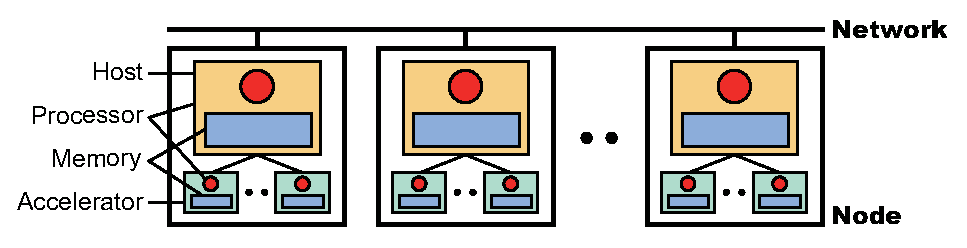
\includegraphics[width=\textwidth]{figs/hardware.eps}
  \caption{Hardware Model}\label{fig:hardware}
\end{myfigure}

An execution unit is called {\bf node} as with {\XMP}.
Each {\bf node} consists of a single host and multiple accelerators (such as GPUs and Intel MICs).
Each host has a processor, which may have several cores, and own local memory.
Each accelerator also has them.
Each {\bf node} is connected with each other via network.
Each {\bf node} can access its local memories directly and remote memories,
that is, the memories of another {\bf node} indirectly.
In a host,
the accelerator memory may be physically and/or virtually separate from the host memory as with the memory model of {\OACC}.
Thus,
a host may not be able to read or write the accelerator memory directly.

\subsection{Programming Model}
{\XACC} is a directive-based language extension based on Fortran 90 and ISO C90 (ANSI C90).
To develop applications on accelerated clusters with ease,
{\XACC} extends {\XMP} and {\OACC} independently as follow:
(1) {\XMP} extensions are to facilitate cooperation between {\XMP} and {\OACC} directives.
(2) {\OACC} extensions are to deal with multiple accelerators.

\subsubsection{{\XMP} Extensions}
In a program using the {\XMP} extensions,
{\XMP}, {\OACC}, and {\XACC} directives are used.
Fig. \ref{fig:concept} shows a concept of the {\XMP} extensions.

\begin{myfigure}
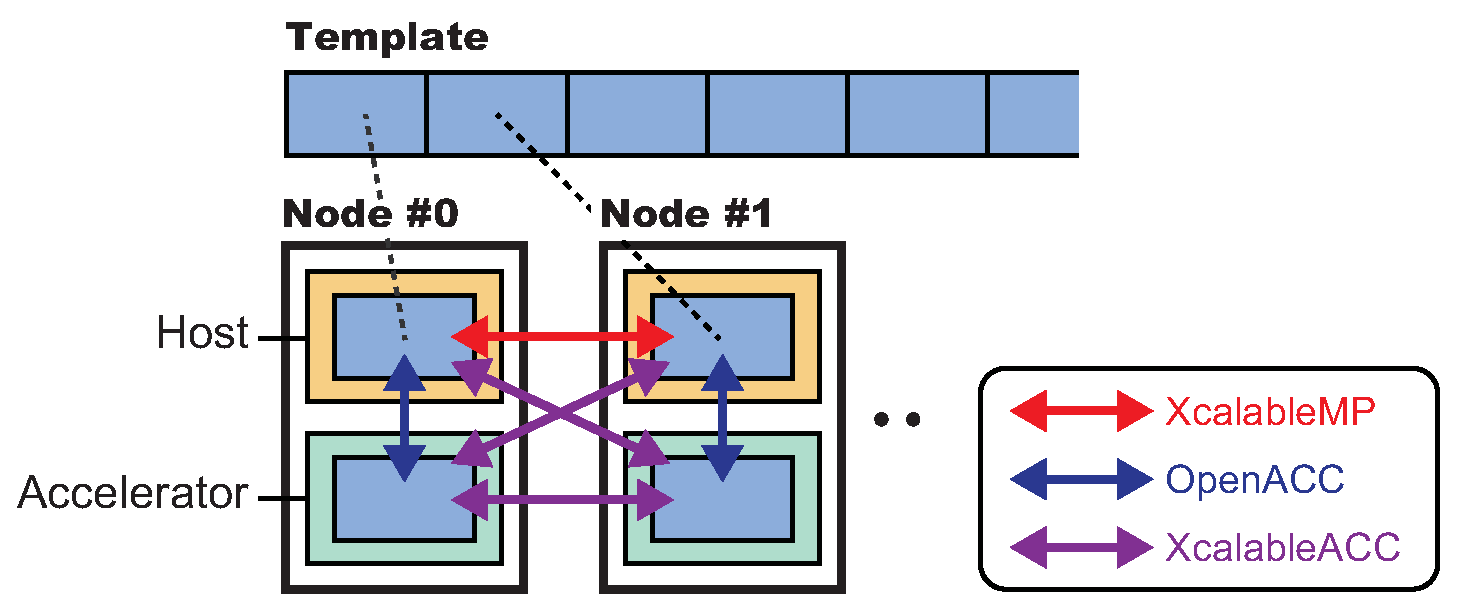
\includegraphics[width=\textwidth]{figs/concept.eps}
  \caption{Concept of {\XMP} Extensions}\label{fig:concept}
\end{myfigure}

{\XMP} directives define a {\bf template} and a {\bf node set}.
The {\bf template} represents a global index space, which is distributed onto the {\bf node set}.
Moreover, {\XMP} directives declare {\bf distributed arrays},
parallelize loop statements and transfer data among host memories according to the distributed {\bf template}.
{\OACC} directives transfer the {\bf distributed arrays} between host memory and accelerator memory on the same {\bf node}
and execute the loop statements parallelized by {\XMP} on accelerators in parallel.
{\XACC} directives, which are {\XMP} communication directives with an {\tt acc} clause, 
transfer data among accelerator memories and between accelerator memory and host memory on different {\bf nodes}.
Moreover, 
{\bf coarray} features also transfer data on different nodes.

%The {\XMP} extension is defined to develop parallel applications with keeping the sequential code image.
Note that 
the {\XMP} extensions are not a simple combination of {\XMP} and {\OACC}.
For example, 
if you represent communication of {\bf distributed array} among accelerators shown in Fig. \ref{fig:concept} by the combination of {\XMP} and {\OACC},
you need to specify explicitly communication between host and accelerator by {\OACC} and that between hosts by {\XMP}.
Moreover,
you need to calculate manually indices of the {\bf distributed array} owned by each {\bf node}.
By contrast,
{\XACC} directives can represent such communication among accelerators directly using global indices.

\subsubsection{{\OACC} Extensions}
The {\OACC} extension can represent offloading works and data to multiple-accelerators on a {\bf node}.
Fig. \ref{fig:concept_acc_ex} shows a concept of the {\OACC} extension.

\begin{myfigure}
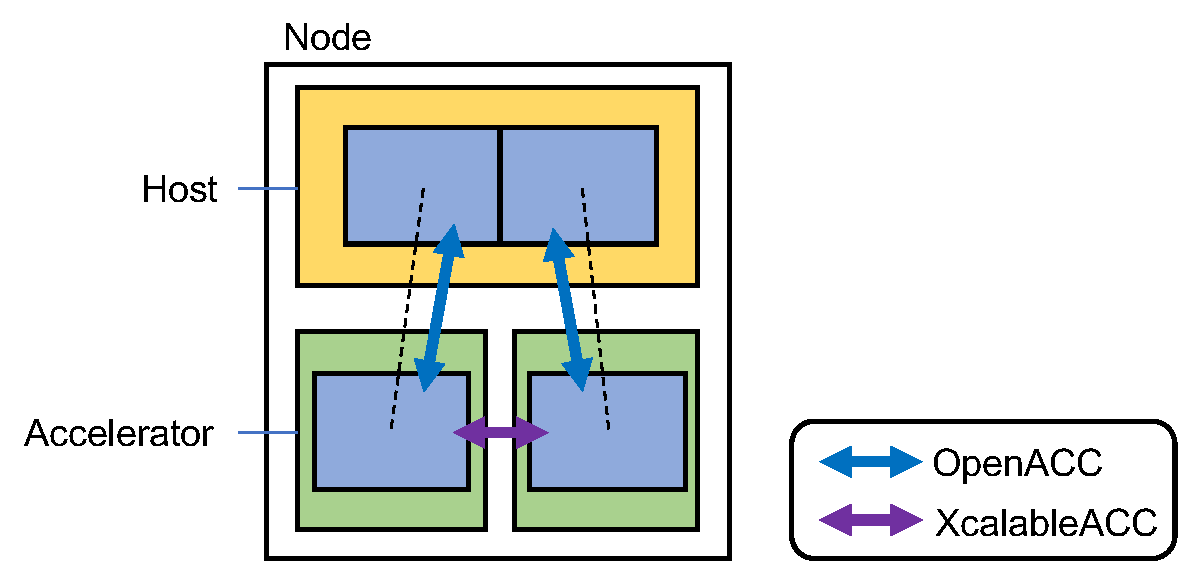
\includegraphics[width=\textwidth]{figs/concept_acc_ext.pdf}
  \caption{Concept of {\OACC} Extension}\label{fig:concept_acc_ex}
\end{myfigure}

{\OACC} extension directive defines a {\bf device set}.
The {\bf device set} represents a set of devices on a {\bf node}.
Futher, {\OACC} extension directives declare {\bf distributed arrays} on the {\bf device set} while maintaining the arrays on the host memory, and the directives distribute offloading loop statement and memory copy between host and device memories for the {\bf distributed-arrays}.
Moreover, {\OACC} extension directives synchronizes devices among the {\bf device set}.
{\XACC} directives also transfer data between device memories on the {\bf node}.

\subsection{Execution Model}
The execution model of {\XACC} is a combination of those of {\XMP} and {\OACC}.
While the execution model of a host CPU programming is based on that of {\XMP},
that of an accelerator programming is based on that of {\OACC}.
Unless otherwise specified,
each {\bf node} behaves exactly as specified in the {\XMP} specification\cite{xmp} or the {\OACC} specification\cite{openacc}.
%For details, refer to each specification\cite{xmp,openacc}.

An {\XACC} program execution is based on the SPMD model, 
where each {\bf node} starts execution from the same main routine and keeps executing the same code independently (i.e. asynchronously), 
which is referred to as the replicated execution
until it encounters an {\XMP} construct or an {\XMP}-extension construct.
In particular,
the {\XMP}-extension construct may allocate, deallocate, or transfer data on accelerators.
An {\OACC} construct or an {\OACC}-extension construct may define {\bf parallel regions}, such as work-sharing loops, 
and offloads it to accelerators under control of the host.

When a {\bf node} encounters a loop construct 
targeted by a combination of {\XMP} {\tt loop} and {\OACC} {\tt loop} directives,
it executes the loop construct in parallel with other {\bf accelerators},
so that each iteration of the loop construct is independently executed by the {\bf accelerator}
where a specified data element resides.

When a {\bf node} encounters a {\XACC} synchronization or a {\XACC} communication directive,
synchronization or communication occurs between it and other accelerators.
That is, such {\bf global constructs} are performed collectively by the {\bf current executing nodes}.
Note that neither synchronizations nor communications occur without these constructs specified.

\subsection{Data Model}
There are two classes of data in {\XACC}: {\bf global data} and {\bf local data} as with {\XMP}. 
Data declared in an {\XACC} program are local by default.
Both {\bf global data} and {\bf local data} can exist on host memory and accelerator memory.
About the data models of host memory and accelerator memory, refer to the OpenACC specification\cite{openacc}.

{\bf Global data} are ones that are distributed onto the {\bf executing node set} by the {\tt align} directive.
Each fragment of a {\bf global data} is allocated in host memory of a {\bf node} in the {\bf executing node set}.
{\OACC} directives can transfer the fragment from host memory to accelerator memory.

{\bf Local data} are all of the ones that are not global.
They are replicated in the local memory of each of the {\bf executing nodes}.

A {\bf node} can access directly only {\bf local data} and sections of {\bf global data} that are allocated in its local memory.
To access data in remote memory, 
explicit communication must be specified in such ways as the global communication constructs and the {\bf coarray} assignments.

Particularly in {\XACCF}, 
for common blocks that include any global variables, 
the ways how the storage sequence of them is defined and how the storage association of them is resolved are implementation-dependent.

% \subsection{Directive Format}
% This section describes the syntax and behavior of {\XMP} and {\OACC} directives in {\XACC}.
% In this document, 
% the following notation is used to describe the directives.

% \vspace{0.5cm}%
% \begin{tabular}{ll}
% {\tt xxx} & {\tt type-face} characters are used to indicate literal type characters. \\
% {\it xxx...} & If the line is followed by ``...'', then xxx can be repeated. \\
% {\it [xxx]} & {\it xxx} is optional. \\
% {\bsquare} & The syntax rule continues. \\
% \verb![F]! & The following lines are effective only in {\XACCF}. \\
% \verb![C]! & The following lines are effective only in {\XACCC}. \\
% \end{tabular}
% \vspace{0.5cm}%

% In {\XACCF}, 
% {\XMP} and {\OACC} directives are specified using special comments that are identified by unique sentinels {\tt\verb|!$xmp|} and {\tt\verb|!$acc|} respectively.
% the directives follow the rules for comment lines of either the Fortran free or fixed source form,
% depending on the source form of the surrounding program unit\footnote{Consequently, the rules of comment lines that an
% {\XMP} directive follows is the same as the ones that an {\OMP} directive follows.}.
% The directives are case-insensitive.

% \vspace{0.5cm}
% \Syntax{directive}
% \begin{tabular}{ll}
% \verb![F]! & \verb|!$xmp| {\it directive-name clause} \\
% \verb![F]! & \verb|!$acc| {\it directive-name clause} \\
% \end{tabular}
% \vspace{0.5cm}

% In {\XACC}, 
% {\XMP} and {\OACC} directives are specified using the \verb|#pragma| mechanism provided by the C standards.
% the directives are case-sensitive.

% \vspace{0.5cm}
% \Syntax{directive}
% \begin{tabular}{ll}
% \verb![C]! & \verb|#pragma xmp| {\it directive-name clause} \\
% \verb![C]! & \verb|#pragma acc| {\it directive-name clause} \\
% \end{tabular}
% \vspace{0.5cm}

%Directives are classified as {\bf declarative directives} and {\bf executable directives}\cite{xmp}.
%
%The {\bf declarative directives} are {\tt nodes}, {\tt template}, {\tt distribute}, {\tt align},
%{\tt shadow}, {\tt coarray}, {\tt declare}, and {\tt routine} directives.
%
%The {\bf executable directives} are {\tt template\_fix}, {\tt task}, {\tt tasks}, {\XMP} {\tt loop}, 
%{\tt array}, {\tt reflect}, {\tt reflect\_init}, {\tt reflect\_do}, {\tt gmove}, {\tt barrier}, 
%{\tt reduction}, {\tt bcast}, {\tt wait\_async},
%{\tt parallel}, {\tt kernels}, {\tt data}, {\tt host\_data}, {\OACC} {\tt loop},
%{\tt cache}, {\tt atomic}, {\tt init}, {\tt shutdown}, {\tt set}, {\tt update}, 
%{\tt wait}, {\tt enter\_data}, and {\tt exit\_data} directives.
%An {\bf executable directive} and its associated user code make up an {\XACC} construct, 
%as in the following format:
%
%\vspace{0.5cm}
%\begin{tabular}{ll}
%\verb![F]! & \verb|!$xmp| {\it directive-name clause} ...\\
% & \hspace{0.5cm} {\it structured-block} \\
%\verb![F]! & \verb|!$acc| {\it directive-name clause} ...\\
% & \hspace{0.5cm} {\it structured-block} \\
%\end{tabular}
%
%\vspace{0.3cm}
%
%\begin{tabular}{ll}
%\verb![C]! & \verb|#pragma xmp| {\it directive-name clause} ...\\
% & \hspace{0.5cm} {\it structured-block} \\
%\verb![C]! & \verb|#pragma acc| {\it directive-name clause} ...\\
% & \hspace{0.5cm} {\it structured-block} \\
%\end{tabular}
%\vspace{0.5cm}

% \subsection{Organization of This Document}
% The remainder of this document is structured as follows:

% \begin{itemize}
%  \item Chapter 2: {\XMP} Extensions
%  \item Chapter 3: {\OACC} Extensions
% \end{itemize}
 %\cleardoublepage
\section{XcalableACC Language}

{\XACC} is roughly defined as a diagonal integration of XMP
and OpenACC with some additional XACC extensions, where XMP directives
are for specifying distributed-memory parallelism, OpenACC for
offloading, and the extensions for other XACC-specific features.

The syntax and semantics of XMP and OpenACC directives appearing in XACC
codes follow those in XMP and OpenACC, respectively, unless specified
below.

\subsection{Data Mapping}

This chapter defines a behavior of mixing {\XMP} and {\OACC}.
Note that the existing {\OACC} is not extended in the {\XMP} extensions.
The {\XMP} extensions can represent 
(1) parallelization with keeping sequential code image using a
combination of {\XMP} and {\OACC}, 
and
(2) communication among accelerator memories and between accelerator
memory and host memory on different {\bf nodes}
using {\XACC} directives or {\bf coarray} features.

% \subsection{Combination of {\XMP} and {\OACC}}

% \subsubsection{{\OACC} Directives on Data}

% \subsubsection*{Description}

When {\bf distributed arrays} appear in {\OACC} constructs,
global indices in {\bf distributed arrays} are used.
The {\bf distributed arrays} may appear in the {\tt update}, {\tt enter
data}, {\tt exit data}, 
{\tt host\_data}, {\tt cache}, and {\tt declare} directives,
and the {\tt data} clause accompanied by some of 
{\tt deviceptr}, {\tt present}, {\tt copy}, {\tt copyin}, 
{\tt copyout}, {\tt create}, and {\tt delete} clauses.
Data transfer of {\bf distributed array} by {\OACC} is performed on only
{\bf nodes} which have elements specified by the global indices.

\subsubsection*{Example}
\begin{myfigure}
\begin{minipage}{0.45\hsize}
\begin{center}
\begin{XACCFexampleL}
integer :: a(N), b(N)
!$xmp template t(N)
!$xmp nodes p(*)
!$xmp distribute t(block) onto p
!$xmp align a(i) with t(i)
!$xmp align b(i) with t(i)
...
!$acc enter data copyin(a(1:K))
!$acc data copy(b)
...
\end{XACCFexampleL}
\end{center}
\end{minipage}
%
\begin{minipage}{0.53\hsize}
\begin{center}
\begin{XACCCexampleR}
int a[N], b[N];
#pragma xmp template t[N]
#pragma xmp nodes p[*]
#pragma xmp distribute t[block] onto p
#pragma xmp align a[i] with t[i]
#pragma xmp align b[i] with t[i]
...
#pragma acc enter data copyin(a[0:K])
#pragma acc data copy(b)
{ ...
\end{XACCCexampleR}
\end{center}
\end{minipage}
\caption{Code example in {\XMP} extensions with {\tt enter\_data}
  directive}\label{code:ex-oacc-data}
\end{myfigure}

In lines 2-6 of Fig. \ref{code:ex-oacc-data},
the directives declare the {\bf distributed arrays} {\it a} and {\it b}.
In line 8,
the {\tt enter data} directive transfers the certain range of the {\bf
distributed array} {\it a} from host memory to accelerator memory. 
Note that the range is represented by global indices.
In line 9,
the {\tt data} directive transfers the whole {\bf distributed array}
{\it b} from host memory to accelerator memory. 


\subsection{Work Mapping}

\subsubsection*{Description}
In order to perform a loop statement on accelerators in {\bf nodes} in parallel,
{\XMP} {\tt loop} directive and {\OACC} {\tt loop} directive are used.
While
{\XMP} {\tt loop} directive performs a loop statement in {\bf nodes} in parallel,
{\OACC} {\tt loop} directive also performs the loop statement
parallelized by the {\XMP} {\tt loop} directive 
on accelerators in parallel.
For ease of writing,
the order of {\XMP} {\tt loop} directive and {\OACC} {\tt loop} directive does not matter.

When {\tt acc} clause appears in {\XMP} loop directive with {\tt reduction} clause,
the directive performs a reduction operation for a variable specified in
the {\tt reduction} clause on accelerator memory.

\subsubsection*{Restriction}
\begin{itemize}
\item In {\OACC} {\bf compute region},
only {\XMP} {\tt loop} directive without {\tt reduction} clause can be inserted.
\item In {\OACC} {\bf compute region},
targeted loop condition (lower bound, upper bound, and step of the loop)
	  must remain unchanged. 
\item {\tt acc} clause in {\XMP} loop directive can appear only when
	  {\tt reduction} clause appears there.
\end{itemize}

\subsubsection*{Example 1}
\begin{myfigure}
\begin{minipage}{0.45\hsize}
\begin{center}
\begin{XACCFexampleL}
integer :: a(N), b(N)
!$xmp template t(N)
!$xmp nodes p(*)
!$xmp distribute t(block) onto p
!$xmp align a(i) with t(i)
!$xmp align b(i) with t(i)
...
!$acc parallel loop copy(a, b)
!$xmp loop on t(i)
do i=0, N
  b(i) = a(i)
end do
!$acc end parallel
\end{XACCFexampleL}
\end{center}
\end{minipage}
%
\begin{minipage}{0.53\hsize}
\begin{center}
\begin{XACCCexampleR}
int a[N], b[N];
#pragma xmp template t[N]
#pragma xmp nodes p[*]
#pragma xmp distribute t[block] onto p
#pragma xmp align a[i] with t[i]
#pragma xmp align b[i] with t[i]
...
#pragma acc parallel loop copy(a, b)
#pragma xmp loop on t[i]
for(int i=0;i<N;i++){
  b[i] = a[i];
}

\end{XACCCexampleR}
\end{center}
\end{minipage}
\caption{Code example in {\XMP} extensions with {\OACC} loop
  construct}\label{code:ex-oacc-loop}
\end{myfigure}

In lines 2-6 of Fig. \ref{code:ex-oacc-loop},
the directives declare {\bf distributed arrays} {\it a} and {\it b}.
In line 8,
the {\tt parallel} directive with the {\tt data} clause transfers the
{\bf distributed arrays} {\it a} and {\it b} from host memory to
accelerator memory.
Moreover,
in lines 8-9,
the {\tt parallel} directive and {\XMP} {\tt loop} directive perform the
next loop statement on accelerators in {\bf nodes} in parallel.

\subsubsection*{Example 2}
\begin{myfigure}
\begin{center}
\begin{XACCFexampleL}
integer :: a(N), sum = 10
!$xmp template t(N)
!$xmp nodes p(*)
!$xmp distribute t(block) onto p
!$xmp align a(i) with t(i)
...
!$acc parallel loop copy(a, sum) reduction(+:sum)
!$xmp loop on t(i) reduction(+:sum) acc
do i=0, N
  sum = sum + a(i)
end do
!$acc end parallel loop
\end{XACCFexampleL}
\begin{XACCCexampleL}
int a[N], sum = 10;
#pragma xmp template t[N]
#pragma xmp nodes p[*]
#pragma xmp distribute t[block] onto p
#pragma xmp align a[i] with t[i]
...
#pragma acc parallel loop copy(a, sum) reduction(+:sum)
#pragma xmp loop on t[i] reduction(+:sum) acc
for(int i=0;i<N;i++){
  sum += a[i];
}
\end{XACCCexampleL}
\end{center}
\caption{Code example in {\XMP} extensions with {\OACC} loop construct
  with reduction clause}\label{code:ex-oacc-loop-reduction}
\end{myfigure}

In lines 2-5 of Fig. \ref{code:ex-oacc-loop-reduction},
the directives declare {\bf distributed array} {\it a}.
In line 7,
the {\tt parallel} directive with the {\tt data} clause transfers the
{\bf distributed array} {\it a} and variable {\bf sum} from host memory
to accelerator memory.
Moreover,
in lines 7-8,
the {\tt parallel} directive and {\XMP} {\tt loop} directive perform the
next loop statement on accelerators in {\bf nodes} in parallel.
When finishing the calculation of the loop statement,
OpenACC {\tt reduction} clause and {\XMP} {\tt reduction} and {\tt acc}
clauses in lines 7-8 perform a reduction operation for the variable {\bf
sum} on accelerators in {\bf nodes}.


\subsection{Data Communication and Synchronization}

\subsubsection{{\tt acc} clause}

\subsubsection{Coarray}

\subsection{Handling Multiple Accelerators}

 -- devices Directive

 -- on\_device Clause

 -- layout Clause

 -- shadow Clause

 -- barrier\_device Construct
 %\cleardoublepage
\section{Omni XcalableACC Compiler}

 %\cleardoublepage
\section{Performance of Lattice QCD Application}

This section describes the evaluations of XACC performance and productivity for a lattice quantum chromodynamics (Lattice QCD) application.

\subsection{Overview of Lattice QCD}
The Lattice QCD is a discrete formulation of QCD that describes the strong interaction among ``quarks'' and ``gluons.''
While the quark is a species of elementary particles, the gluon is a particle that mediates the strong interaction.
The Lattice QCD is formulated on a four-dimensional lattice (time: T and space:ZYX axes).
We impose a periodic boundary condition in all the directions.
The quark degree of freedom is represented as a field that has four components of ``spin'' and three components of ``color,''
namely a complex vector of $12 \times N_{site}$ components,
where $N_{site}$ is the number of lattice sites.
The gluon is defined as a $3\times 3$ complex matrix field on links (bonds between neighboring lattice sites).
During a Lattice QCD simulation,
one needs to solve many times a linear equation for the matrix that represents the interaction between the quark and gluon fields.
This linear equation is the target of present work.
The matrix acts on the quark vector and has nonzero components only for the neighboring sites, and thus sparse.

\subsection{Implementation}
We implemented a Lattice QCD code based on the existing Lattice QCD application Bridge++\cite{bridge++}.
Since our code was implemented by extracting the main kernel of the Bridge++,
it can be used as a mini-application to investigate its productivity and performance more easily than
use of the original Bridge++.

\begin{figure}[h]
\centering
\begin{minipage}{0.45\hsize}
\begin{lstlisting}
S = B
R = B
X = B
sr = norm(S)
T = WD(U,X)
S = WD(U,T)
R = R - S
P = R
rr = norm(R)
rrp = rr
do{
\end{lstlisting}
\end{minipage} \hspace{0.5cm}
\begin{minipage}{0.45\hsize}
\begin{lstlisting}[firstnumber=10]
  T = WD(U,P)
  V = WD(U,T)
  pap = dot(V,P)
  cr = rr/pap
  X = cr * P + X
  R = -cr * V + R
  rr = norm(R)
  bk = rr/rrp
  P = bk * P + R
  rrp = rr
}while(rr/sr > 1.E-16)
\end{lstlisting}
\end{minipage}
\caption{Lattice QCD pseudo code}\label{fig:pseudo}
\end{figure}

Fig. \ref{fig:pseudo} shows a pseudo code of the implementation,
where the CG method is used to solve quark propagators.
In Fig. \ref{fig:pseudo},
{\it WD()} is the Wilson-Dirac operator\cite{PhysRevD.10.2445},
{\it U} is a gluon, the other uppercase characters are quarks.
The Wilson-Dirac operator is a main kernel in the Lattice QCD,
which calculates how the quarks interact with each other under the influence of the gluon.

\begin{figure}[h]
\centering
\begin{lstlisting}
typedef struct Quark {
 double v[4][3][2];
} Quark_t;
typedef struct Gluon {
 double v[3][3][2];
} Gluon_t;
Quark_t v[NT][NZ][NY][NX], tmp_v[NT][NZ][NY][NX];
Gluon_t u[4][NT][NZ][NY][NX];

#pragma xmp template t[NT][NZ]
#pragma xmp nodes n[NODES_T][NODES_Z]
#pragma xmp distribute t[block][block] onto n
#pragma xmp align v[i][j][*][*] with t[i][j]
#pragma xmp align tmp_v[i][j][*][*] with t[i][j]
#pragma xmp align u[*][i][j][*][*] with t[i][j]
#pragma xmp shadow v[1:1][1:1][0][0]
#pragma xmp shadow tmp_v[1:1][1:1][0][0]
#pragma xmp shadow u[0][1:1][1:1][0][0]
...
int main(){
...
#pragma acc enter data copyin(v, tmp_v, u)
\end{lstlisting}
\caption{Declaration of distributed arrays for Lattice QCD}\label{fig:distributedQCD}
\end{figure}

Fig. \ref{fig:distributedQCD} shows how to declare distributed arrays of the quark and gluon.
In lines 1-8, the quark and gluon structure arrays are declared.
The last dimension ``[2]'' of both structures represents real and imaginary parts for a complex number.
{\it NT}, {\it NZ},  {\it NY} and {\it NX} are the numbers of TZYX axis elements.
In lines 10-18, distributed arrays are declared where the macro constant values {\it NODES\_T} and {\it NODES\_Z} indicate the number of {\tt nodes} on the T and Z axes.
Thus,
the program is parallelized on T and Z axes.
Note that an ``*'' in the {\bf align} directive means that the dimension is not divided.
In the {\bf shadow} directive,
halo regions are added to the arrays because each quark and gluon element is affected by its neighboring orthogonal elements.
Note that ``0'' in the {\bf shadow} directive means that no halo region exists.
In line 22,
the {\bf enter data} directive transfers the distributed arrays from host memory to accelerator memory.

\begin{figure}[h]
\centering
\begin{lstlisting}
#pragma xmp reflect(v) width(/periodic/1:1,/periodic/1:1,0,0) orthogonal acc
#pragma xmp reflect(u) width(0,/periodic/1:0,/periodic/1:0,0,0) orthogonal acc
WD(tmp_v, u, v);
#pragma xmp reflect(tmp_v) width(/periodic/1:1,/periodic/1:1,0,0) orthogonal acc
WD(v, u, tmp_v);
\end{lstlisting}
\caption{Calling Wilson-Dirac operator}\label{fig:callingDirac}
\end{figure}

Fig. \ref{fig:callingDirac} shows how to call {\it WD()}.
The  {\bf reflect} directives are inserted before {\it WD()} in order to update own halo region.
In line 2,
``1:0'' in {\bf width} clause means only the lower halo region is updated because only it is needed in {\it WD()}.
The {\it u} is not updated before the second {\it WD()} function because values of {\it u} are not updated in {\it WD()}.
Moreover,
the {\bf orthogonal} clause is added because diagonal updates of the arrays are not required in {\it WD()}.

\begin{figure}[h]
\centering
\begin{lstlisting}
void WD(Quark_t v_out[NT][NZ][NY][NX], const Gluon_t u[4][NT][NZ][NY][NX], const Quark_t v[NT][NZ][NY][NX])
{
#pragma xmp align v_out[i][j][*][*] with t[i][j]
#pragma xmp align u[*][i][j][*][*] with t[i][j]
#pragma xmp align v[i][j][*][*] with t[i][j]
#pragma xmp shadow v_out[1:1][1:1][0][0]
#pragma xmp shadow u[0][1:1][1:1][0][0]
#pragma xmp shadow v[1:1][1:1][0][0]
 ...
#pragma xmp loop (t,z) on t[t][z]
#pragma acc parallel loop collapse(4) present(v_out, u, v)
 for(int t=0;t<NT;t++)
  for(int z=0;z<NZ;z++)
   for(int y=0;y<NY;y++)
    for(int x=0;x<NX;x++){
\end{lstlisting}
\caption{A portion of Wilson-Dirac operator}\label{fig:dirac}
\end{figure}

Fig. \ref{fig:dirac} shows a part of the Wilson-Dirac operator code.
All arguments in {\it WD()} are distributed arrays.
In XMP and XACC,
distributed arrays which are used as arguments must be redeclared in function to pass their information to a compiler.
Thus, the {\bf align} and {\bf shadow} directives are used in {\it WD()}.
In line 10, the {\bf loop} directive parallelizes the outer two loop statements.
In line 11, the {\bf parallel loop} directive parallelizes all loop statements.
In the loop statements,
a calculation needs neighboring and orthogonal elements.
Note that while the {\it WD()} updates only the {\it v\_out},
it only refers the {\it u} and {\it v}.

\begin{figure}[h]
\centering
\begin{lstlisting}
double norm(const Quark_t v[NT][NZ][NY][NX])
{
#pragma xmp align v[i][j][*][*] with t[i][j]
#pragma xmp shadow v[1:1][1:1][0][0]
 double a = 0.0;

#pragma xmp loop (t,z) on t[t][z]
#pragma acc parallel loop collapse(7) present(v) reduction(+:a)
 for(int t=0;t<NT;t++)
  for(int z=0;z<NZ;z++)
   for(int y=0;y<NY;y++)
    for(int x=0;x<NX;x++)
     for(int i=0;i<4;i++)
      for(int j=0;j<3;j++)
       for(int k=0;k<2;k++)
        a += v[t][z][y][x].v[i][j][k]*v[t][z][y][x].v[i][j][k];

#pragma xmp reduction (+:a)
 return a;
}
\end{lstlisting}
\caption{L2 norm calculation code}\label{fig:norm}
\end{figure}

Fig. \ref{fig:norm} shows L2 norm calculation code in the CG method.
In line 8,
the {\bf reduction} clause performs a reduction operation for the variable {\it a} in each accelerator when finishing the next loop statement.
The calculated variable {\it a} is located in both host memory and accelerator memory.
However, at this point,
all {\tt nodes} have individual values of {\it a}.
To obtain the total value of the variable {\it a},
the XMP {\bf reduction} directive in line 18 also performs a reduction operation among {\tt nodes}.
Since the total value is used on only host after this function,
the XMP {\bf reduction} directive does not have {\bf acc} clause.

\section{Performance Evaluation}\label{sec:performance}
\subsection{Result}
\begin{table}[h]
\renewcommand{\arraystretch}{1.2}
\centering
\caption{Evaluation environment} \label{tab:ha-pacs/tca}
\begin{tabular}{l|l}\hline
CPU & Intel Xeon-E5 2680v2 2.8 GHz x 2 Sockets \\
Memory & DDR3 1866MHz 59.7GB/s 128GB \\
GPU & NVIDIA Tesla K20X (GDDR5 250GB/s 6GB) x 4 GPUs \\
Network & InfiniBand Mellanox Connect-X3 Dual-port QDR 8GB/s \\
\multirow{2}{*}{Software} & Intel 16.0.2, CUDA 7.5.18, Omni OpenACC compiler 1.1\\
 & MVAPICH2 2.1\\ \hline
\end{tabular}
\end{table}

This section evaluates the performance level of XACC on the Lattice QCD code.
For comparison purposes,
those of MPI+CUDA and MPI+OpenACC are also evaluated.
For performance evaluation,
we use the HA-PACS/TCA system\cite{hapacs} the hardware specifications and software environments of which are shown in Table \ref{tab:ha-pacs/tca}.
Since each compute node has four GPUs,
we assign four {\tt nodes} per compute node and direct each {\tt node} to deal with a single GPU.
We use the Omni OpenACC compiler\cite{2013tabuchi} as a backend compiler in the Omni XACC compiler.
We execute the Lattice QCD codes with strong scaling in regions (32,32,32,32) as ({\it NT},{\it NZ},{\it NY},{\it NX}).
The Omni XACC compiler provides various types of data communication among accelerators\cite{nakao2014}.
We use the MPI+CUDA implementation type because it provides a balance of versatility and performance.

\begin{figure}[h]
\centering
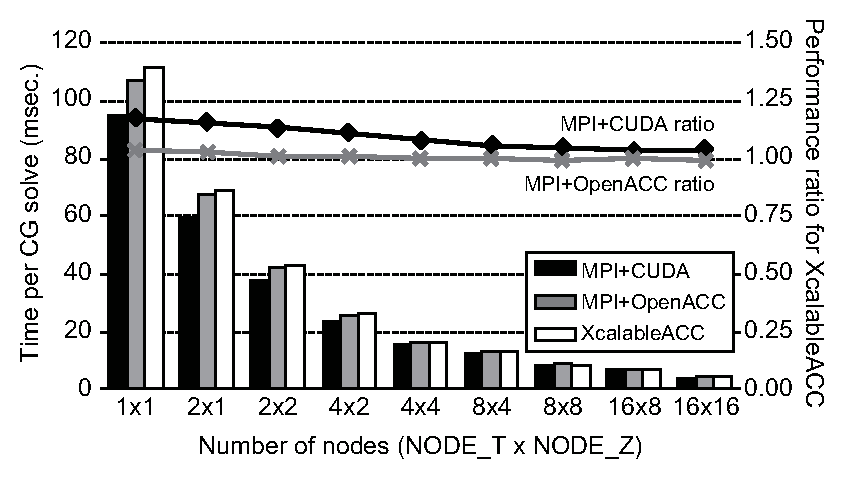
\includegraphics[scale=0.58,clip]{figs/performance32.eps}
\caption{Performance results} \label{fig:performance}
\end{figure}

Fig. \ref{fig:performance} shows the performance results that indicate the time required to solve one CG iteration as well as the performance ratio values that indicate the comparative performance \
of XACC and other languages.
When the performance ratio value of a language is greater than 1.00,
the performance result of the language is better than that of XACC.
Fig. \ref{fig:performance} shows that the performance ratio values of MPI+CUDA are between 1.04 and 1.18,
and that those of MPI+OpenACC are between 0.99 and 1.04.
Moreover,
Fig. \ref{fig:performance} also shows that the performance results of both MPI+CUDA and MPI+OpenACC become closer to those of XACC as the number of {\tt nodes} increases.

\subsection{Discussion}
To examine the performance levels in detail,
we measure the time required for the halo updating operation for two {\tt nodes} and more.
The halo updating operation consists of the communication and pack/unpack processes for non-contiguous regions in the XACC runtime.

\begin{figure}[h]
\centering
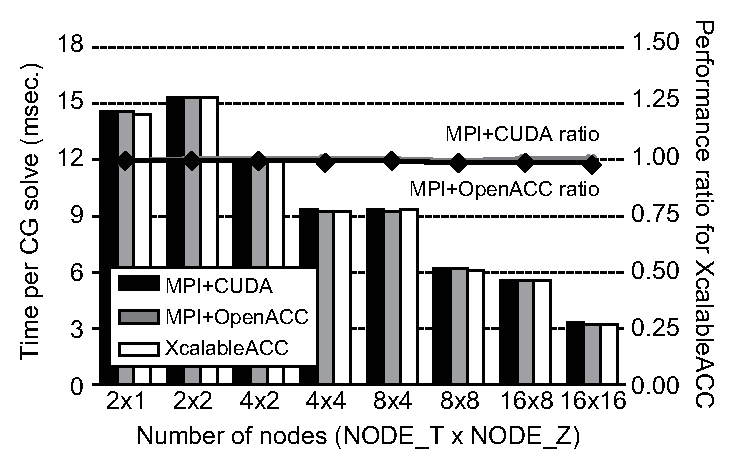
\includegraphics[scale=0.58,clip]{figs/halo-comm.eps}
\caption{Communication time} \label{fig:halo-comm}
\end{figure}

\begin{figure}[h]
\centering
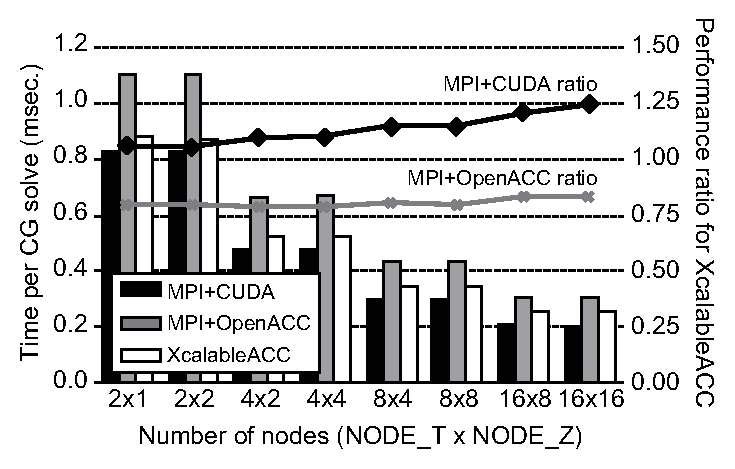
\includegraphics[scale=0.58,clip]{figs/halo-pack-unpack.eps}
\caption{Pack/unpack time} \label{fig:halo-pack-unpack}
\end{figure}

While Fig. \ref{fig:halo-comm} describes communication time of the halo updating time of Fig \ref{fig:performance},
Fig. \ref{fig:halo-pack-unpack} describes pack/unpack time of it.
Fig. \ref{fig:halo-comm} shows that
the communication performance levels of all implementations are almost the same.
However,
Fig. \ref{fig:halo-pack-unpack} shows that the pack/unpack performance levels of MPI+CUDA are better than those of XACC,
and that those of MPI+OpenACC are worse than those of XACC.
The reason for the pack/unpack operation performance level difference is that the XACC operation is implemented in CUDA at XACC runtime.
Thus,
some performance levels of XACC are better than those of MPI+OpenACC in Fig. \ref{fig:performance}.
However,
the performance levels of XACC in Fig. \ref{fig:halo-pack-unpack} is worse than those of MPI+CUDA because XACC requires the cost of XACC runtime calls.

\begin{figure}[h]
\centering
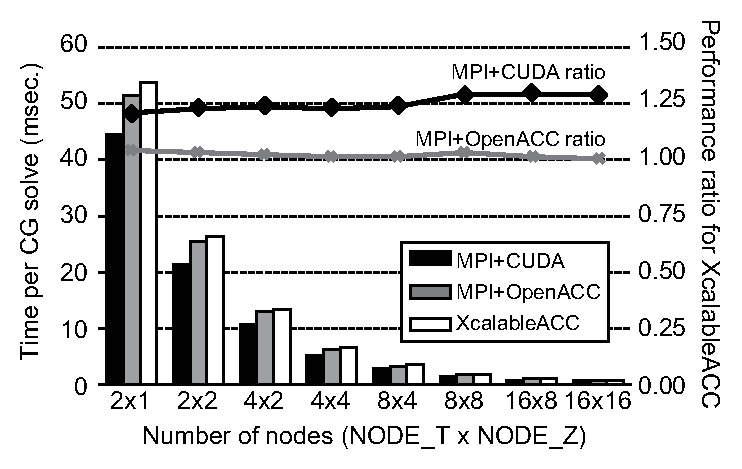
\includegraphics[scale=0.58,clip]{figs/exceptforhalo.eps}
\caption{Time excluding halo updating time} \label{fig:exceptforhalo}
\end{figure}

Fig. \ref{fig:exceptforhalo} shows the overall time excluding the halo updating time,
where performance levels of MPI+CUDA are the best, and those of XACC are almost the same as those of MPI+OpenACC.
The reason for the difference is due to how to use GPU threads.
In the CUDA implementation,
we assign loop iterations to GPU threads in a cyclic-manner manually.
In contrast, in the OpenACC and XACC implementations,
how to assign GPU threads is an implementation dependent of an OpenACC compiler.
In the Omni OpenACC compiler,
initially loop iterations are assigned to GPU threads by a gang (threadblock) in a block manner,
and then are also assigned to them by a vector (thread) in a cyclic manner.
With the {\bf gang} clause with the {\bf static} argument proposed in the OpenACC specification version 2.0,
programmers can determine how to use GPU threads to some extent,
but the Omni OpenACC compiler does not yet support it.

\begin{figure}[h]
\centering
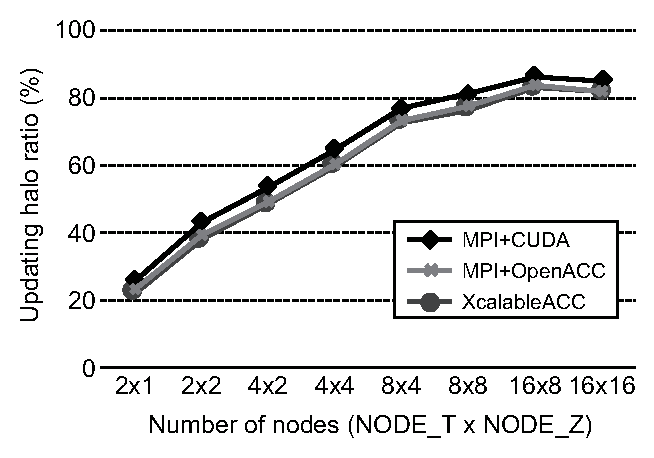
\includegraphics[scale=0.58,clip]{figs/exceptforhalo-per.eps}
\caption{Updating halo ratio} \label{fig:exceptforhalo-per}
\end{figure}

Fig. \ref{fig:exceptforhalo-per} shows the ratio of the halo updating time to overall time.
As can be seen,
as the number of {\tt nodes} increases, the ratio increases as well.
Therefore,
when a large number of {\tt nodes} are used,
there is little difference in performance level of Fig. \ref{fig:performance} among the three implementations.
The reason why the ratio of MPI+CUDA is slightly larger than those of the others is that
the time excluding the halo communication of MPI+CUDA in Fig. \ref{fig:halo-comm} is relatively small.

\section{Productivity Improvement}
\subsection{Requirement for Productive Parallel Language}
\begin{figure}[h]
\centering
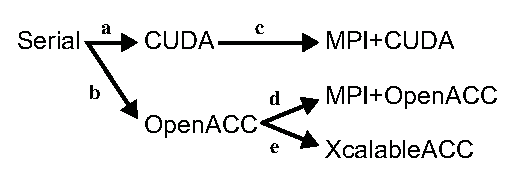
\includegraphics[scale=0.75,clip]{figs/howtocreate1.eps}
\caption{Application development order on accelerated cluster} \label{fig:howtocreate}
\end{figure}

In Section \ref{sec:performance},
we developed three Lattice QCD codes using MPI+CUDA, MPI+OpenACC, and XACC.
Fig. \ref{fig:howtocreate} shows our procedure for developing each code where
we first develop the code for an accelerator from the serial code,
and then extend it to handle an accelerated cluster.

To parallelize the serial code for an accelerator using CUDA requires large code changes (``a'' in Fig. \ref{fig:howtocreate}),
most of which are necessary to create new kernel functions and to make 1D arrays out of multi-dimensional arrays.
By contrast,
OpenACC accomplishes the same parallelization with just small code changes (``b''),
because OpenACC's directive-based approach encourages reuse of an existing code.
Besides,
to parallelize the code for a distributed memory system,
MPI also requires large changes (``c'' and ``d''),
primarily to convert global indices into local indices.
By contrast,
XACC requires smaller code changes (``e'') because XACC is also directive-based language as OpenACC.

In many cases,
a parallel code for an accelerated cluster is based on an existing serial code.
The code changes to the existing serial code are likely to trigger program bugs.
Therefore,
XACC is designed to reuse an existing code as possible.

\subsection{Quantitative Evaluation by Delta Source Lines of Codes}
\begin{table}[h]
\renewcommand{\arraystretch}{1.2}
\centering
\caption{DSLOC of Lattice QCD implementations} \label{tab:dsloc}
\begin{tabular}[h]{r|rrrrr|rrr} \hline
       & a   & b  & c   & d   & e   & a+c & b+d & {\bf b+e}  \\ \hline
DSLOC  & 552 & 22 & 280 & 201 & 138 & 832 & 223 & {\bf 160} \\  \hline
Add    & 137 & 20 & 185 & 140 & 134 & 322 & 160 & {\bf 154} \\
Delete & 73 & 0 & 0 & 0 & 0 & 73 & 0 & {\bf 0} \\
Modify & 342 & 2 & 95 & 61 & 4 & 437 & 63 & {\bf 6} \\ \hline
\end{tabular}
\end{table}

As one of metrics for productivity,
Delta Source Lines of Codes (DSLOC) is proposed\cite{CGPOP2011}.
The DSLOC indicates how the codes change from a corresponding implementation.
The DSLOC is the sum of three components: how many lines are added, deleted and modified.
When the DSLOC is small,
the programming costs and the possibility of program bugs will be small as well.
We use the DSLOC to count the amount of change required to implement an accelerated cluster code from a serial code.

Table \ref{tab:dsloc} shows the DSLOC where lowercase characters correspond to Fig. \ref{fig:howtocreate}.
The DSLOC of XACC (b+e) is smaller than MPI+CUDA (a+c) and MPI+OpenACC (b+d).
The difference between XACC and MPI+CUDA is 420.0\%, and that between XACC and MPI+OpenACC is 39.4\%.

\subsection{Discussion}\label{sec:pro-con}
\begin{figure}[h]
\centering
\begin{lstlisting}
#pragma acc parallel loop collapse(4) present(v_out, u, v)
 for(int t=0;t<NT;t++)
  for(int z=0;z<NZ;z++)
   for(int y=0;y<NY;y++)
    for(int x=0;x<NX;x++){
     int tt = (t + 1) % NT;
     v_out[tt][z][y][x].v[0][0][0] = ... ;
\end{lstlisting}\vspace{-1.5ex}
\caption{Code modification of {\it WD()} in OpenACC}\label{fig:modification-openacc}
\end{figure}

\begin{figure}[h]
\centering
\begin{lstlisting}
#pragma xmp loop (t,z) on t[t][z]
#pragma acc parallel loop collapse(4) present(v_out, u, v)
 for(int t=0;t<NT;t++)
  for(int z=0;z<NZ;z++)
   for(int y=0;y<NY;y++)
    for(int x=0;x<NX;x++){
     int tt = t + 1;
     v_out[tt][z][y][x].v[0][0][0] = ... ;
\end{lstlisting}\vspace{-1.5ex}
\caption{Code modification of {\it WD()} in XcalableACC}\label{fig:modification-xacc}
%\caption{Code modification in {\it WD()}} \label{fig:modification}
\end{figure}

In ``e'' of Table \ref{tab:dsloc},
four lines for modification are required to implement the XACC code from the OpenACC code.
Fig. \ref{fig:modification-openacc} and \ref{fig:modification-xacc} show the modification,
which is a part of {\it WD()} of Fig. \ref{fig:dirac}.
A variable {\it tt} is used to be an index for halo region.
The {\it tt} is modified from line 6 of Fig. \ref{fig:modification-openacc} to line 7 of Fig. \ref{fig:modification-xacc}.
In Fig. \ref{fig:modification-openacc},
when a value of a variable {\it t} is ``{\it NT}-1'',
that of the variable {\it tt} becomes ``0'' which is the lower bound index of the first dimension of the array {\it v\_out}.
On the other hand,
in Fig. \ref{fig:modification-xacc},
communication of the halo is performed before execution of {\it WD()} by the {\bf reflect} directive shown in Fig. \ref{fig:callingDirac}.
Thus,
the variable {\it tt} need only be incremented in Fig. \ref{fig:modification-xacc}.
There are four such modifications in {\it WD()}.
Note that
XACC does not keep the semantics of the base code perfectly in this case
in exchange for simplified parallelization.
In addition,
there are two lines for modification shown in ``b'' of Table \ref{tab:dsloc}.
It is a very fine modification for OpenACC constraints,
which keeps the semantics of the base code.

\begin{table}[h]
\renewcommand{\arraystretch}{1.2}
\centering
\caption{SLOC of Lattice QCD implementations} \label{tab:sloc}
\begin{tabular}[h]{r|rrr} \hline
               & MPI+CUDA & MPI+OpenACC & {\bf XcalableACC}  \\ \hline
SLOC           & 1091     & 1002        & {\bf 996} \\ \hline
\#XcalableMP   & -        & -           & {\bf 122} \\
\#OpenACC      & -        & 26          & {\bf 16}  \\
\#XcalableACC  & -        & -           & {\bf 3}   \\
\#MPI function & 39       & 39          & {\bf -}   \\ \hline
\end{tabular}
\end{table}

\begin{figure}[h]
\centering
\begin{lstlisting}
void WD(Quark_t v_out[NT][NZ][NY][NX], const Gluon_t u[4][NT][NZ][NY][NX], const Quark_t v[NT][NZ][NY][NX])
{
#pragma xmp align [i][j][*][*] with t[i][j] shadow [1:1][1:1][0][0] :: v_out, v
#pragma xmp align [*][i][j][*][*] with t[i][j] shadow [0][1:1][1:1][0][0] :: u
\end{lstlisting}
\caption{New directive combination syntax that applies to Fig. \ref{fig:dirac}}\label{fig:combine}
\end{figure}

As basic information,
we count the source lines of codes (SLOC) of each of the Lattice QCD implementations.
Table \ref{tab:sloc} shows the SLOC excluding comments and blank lines,
as well as the numbers of each directive and MPI functions included in their SLOC.
For reader information,
SLOC of the serial version Lattice QCD code is 842.
Table \ref{tab:sloc} shows that
the 122 XMP directives are used in the XACC implementation,
many of which are declarations for function arguments.
To reduce the XMP directives,
we are planning to develop a new syntax that combines declarations with the same attribute into one directive.
Fig. \ref{fig:combine} shows an example of the new syntax applied to the declarations in Fig. \ref{fig:dirac}.
Since the arrays {\it v\_out} and {\it v} have the same attribute,
they can be declared into a single XMP directive.
Moreover,
the {\bf shadow} directive attribute is added to the {\bf align} directive as its clause.
When applying the new directive to XACC implementation,
the number of XMP directives decreases from the 122 shown in Table \ref{tab:sloc} to 64,
and the XACC DSLOC decreases from the 160 shown in Table \ref{tab:dsloc} to 102.
 %\cleardoublepage
%\input{glossary.tex}

% \cleardoublepage
% \chapter*{Acknowledgment}
% %\begin{itemize}
% %\setlength{\itemsep}{-1mm}
% %\item Taisuke Boku       \dotfill \ University of Tsukuba
% %\item Hidetoshi Iwashita \dotfill \ RIKEN/Fujitsu Inc.
% %\item Hitoshi Murai      \dotfill \ RIKEN
% %\item Masahiro Nakao     \dotfill \ RIKEN
% %\item Mitsuhisa Sato     \dotfill \ RIKEN
% %\item Akihiro Tabuchi     \dotfill \ University of Tsukuba
% %\end{itemize}

% The work was supported by the Japan Science and Technology Agency, 
% Core Research for Evolutional Science and Technology program entitled 
% ``Research and Development on Unified Environment of Accelerated Computing and Interconnection for Post-Petascale Era'' 
% in the research area of ``Development of System Software Technologies for Post-Peta Scale High Performance Computing.''

%The specification of {\XMP} is designed by the {\XMP} Specification
%Working Group, which consists of the following members from academia,
%research laboratories, and industries.

\begin{thebibliography}{99}
\addcontentsline{toc}{chapter}{\bibname}
\bibitem{aaa} Masahiro Nakao et al.
 ``Evaluation of XcalableACC with Tightly Coupled Accelerators/InfiniBand Hybrid Communication on Accelerated Cluster'', International Journal of High Performance Computing Applications (2019)
 \bibitem{xmp} XcalableMP Language Specification, \url{http://xcalablemp.org/specification.html} (2017).
 \bibitem{openacc} The OpenACC Application Programming Interface, \url{http://www.openacc.org} (2015).
 \bibitem{mpi} MPI: A Message-Passing Interface Standard, \url{http://mpi-forum.org} (2015).
 \bibitem{bridge++} Lattice QCD code Bridge++, \url{http://bridge.kek.jp/Lattice-code/index\_e.html}.
 \bibitem{PhysRevD.10.2445} Wilson, K. G., ``Confinement of quarks'' (1974).
 \bibitem{hapacs} HA-PACS, \url{https://www.ccs.tsukuba.ac.jp/supercomputer/}.
 \bibitem{2013tabuchi} Akihiro Tabuchi et al, ``A Source-to-Source OpenACC Compiler for CUDA'', Euro-Par Workhops (2013)
 \bibitem{nakao2014} Masahiro Nakao et al. ``XcalableACC: Extension of XcalableMP PGAS Language Using OpenACC for Accelerator Clusters'',
   Proceedings of the First Workshop on Accelerator Programming Using Directives (2014)
 \bibitem{CGPOP2011} Andrew I. Stone et al. ``Evaluating Coarray Fortran with the CGPOP Miniapp'',
   Proceedings of the Fifth Conference on Partitioned Global Address Space Programming Models (2011)
\end{thebibliography}

\end{document}
